\chapter{Architecture}

\section{Overview}

\begin{figure}[h]
    \caption{Overview}
    \centering
    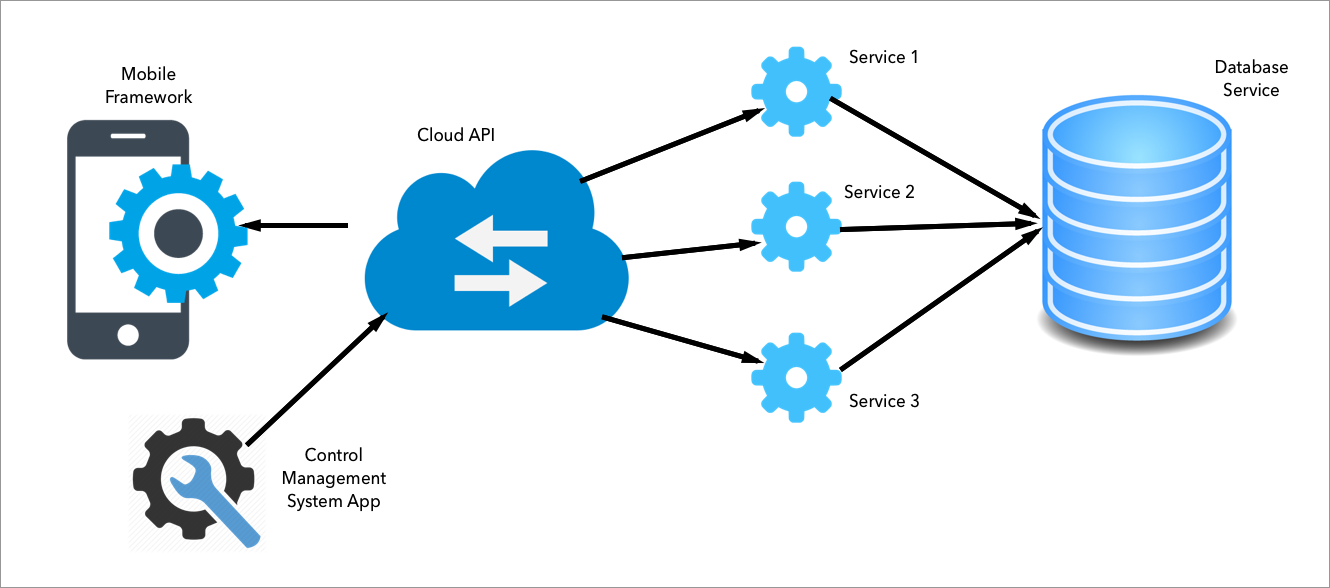
\includegraphics[width=100mm]{images/overview}
    \label{fig:label}
\end{figure}

Figure \ref{fig:label} illustrates the overview architecture of systems and the four main parts. The first being the web- server that provides a cloud-based service, that takes requests and performs the necessary task. The next part which follows on from the web-server is the database, to store data persistently. This also provides a cloud-based database so that data can be accessed from anywhere. The third part being the mobile framework which creates the communication to the web server through an API which will be discussed later in this chapter. The framework separates the complexity of the web-server system and provides easy to use tools to communicate. The last main part is the control management system app, which provides an interface to configure the web- server and display the current set-up.

\section{Web Architecture}

\begin{figure}[!h]
    \caption{Four-tier Architecture \cite{ted} }
    \centering
    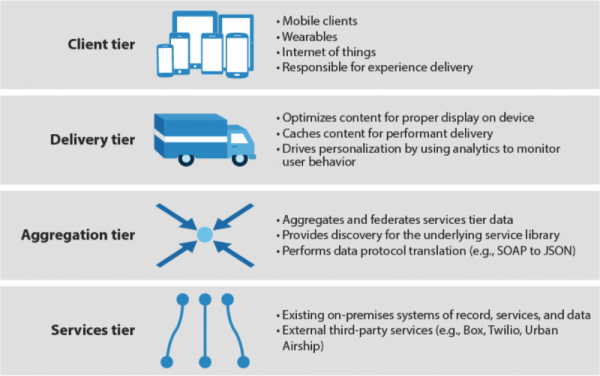
\includegraphics[width=100mm]{images/four-tier}
    \label{fig:four-tier}
\end{figure}

The Four-Tier Engagement Platform is the chosen web architecture for my project shown in Fig \ref{fig:four-tier}. The client tier allows the development of an application without having to worry about the backend services. Delivery tier gives the consumer the best possible mobile experience by caching content locally on the device app, so if service is lost, then they can still use the app. The aggregation tier connects the apps to the right services with bi-directional, real-time data from the back-end. Finally, the service tier gives the other levels the data they require. It is also used to integrate current services already being used by the company such as MySQL or MongoDB.

\section{Back-end as a Service}

\begin{figure}[!h]
    \caption{Client Server Diagram \cite{backendless} }
    \centering
    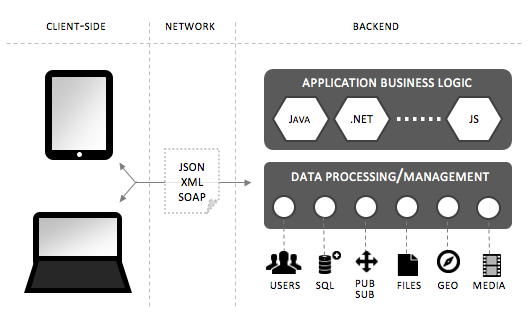
\includegraphics[width=100mm]{images/client-server-diagram}
    \label{fig:client-server}
\end{figure}

Applications today are put into the category of ”client-server apps” where the applications consist of client-side(front-end) and the server-side(backend). The client-side is what the user see, whatever type of device it is, being a computer or mobile apps. The client-side responsibility is showing the data to the user in an easy to read interface, along with taking their requests and passing it to the server. The backend consists of two primary components: application business logic and data processing/management. The data processing/management operates on various resources being users, persistent data, files, etc. The business logic manages triggering notifications based on changes in the data, prevent unauthorised access and figure \ref{fig:client-server} illustrates this.

\section{API}

For the applications to communicate with the back-end, there needs to be a standard-based protocol that defines how data flows. Thus combining the protocol with the data structure definitions creates an Appli- cation Programming Interface (API). The typical format used in most applications is called Representational State Transfer REST which is an architectural style and approach to communications used in web services development. REST provides a list of verbs such as GET, POST, DELETE in which request can be made using HTTP. The diagram \ref{fig:api} below illustrates this.

\begin{figure}[!h]
    \caption{API \cite{backendless}}
    \centering
    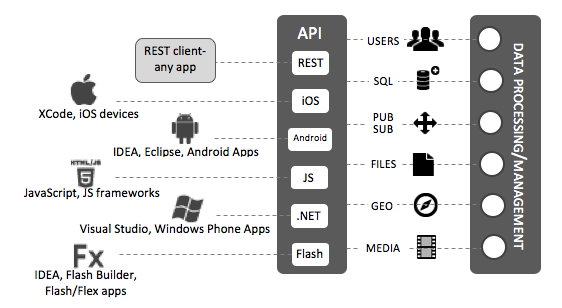
\includegraphics[width=100mm]{images/baas-apis}
    \label{fig:api}
\end{figure}


